\centerline{\bf \huge 8 класс}
\centerline{\bf \huge Решения}

\problem{8.1}
В десятизначном числе пронумеровали слева направо все цифры числами от 1 до 10 , после чего все цифры с чётными номерами в том же порядке переставили на первые пять мест, а все цифры с нечётными номерами в том же порядке переставили на последние 5 мест. Получившееся число совпало с исходным. Какое наибольшее количество различных цифр может быть в таком числе?

\textit{Ответ. 1.}

\textit{Решение.}
Обозначим это десятизначное число через $\overline{a_1 a_2 a_3 a_4 a_5 a_6 a_7 a_8 a_9 a_{10}}$. Тогда по условию оно совпадает с числом $\overline{a_2 a_4 a_6 a_8 a_{10} a_1 a_3 a_5 a_7 a_9}$. Значит, $a_1=a_2=a_4=a_8=a_5=a_{10}=a_9=a_7=a_3=a_6$, то есть все цифры обязаны быть одинаковыми. Число, состоящее из 10 одинаковых цифр, подходит.

\problem{8.2}
На биссектрисе острого угла $A B C$ отмечены точки $D$ и $E$ так, что $A B=B D=A E$ и $D E=B C$ (точка $D$ лежит между $B$ и $E$ ). Докажите, что $A D=C D$.

\textit{Решение.}
Поскольку $A B=A E$, то треугольник $A B E$ равнобедренный, значит $\angle A E B= \angle A B E$, а поскольку $B E$ - биссектриса угла $A B C$, то $\angle A E B=\angle A B E=\angle E B C$. Рассмотрим треугольники $A E D$ и $D B C$. Стороны $A E$ и $B D$, а также $D E$ и $B C$ равны по условию, и углы $A E D$ и $D B C$ равны по ранее доказанному. Значит, эти треугольники равны по первому признаку равенства треугольников. Откуда $A D=C D$, что и требовалось.

\begin{figure}[h]
    \centering
    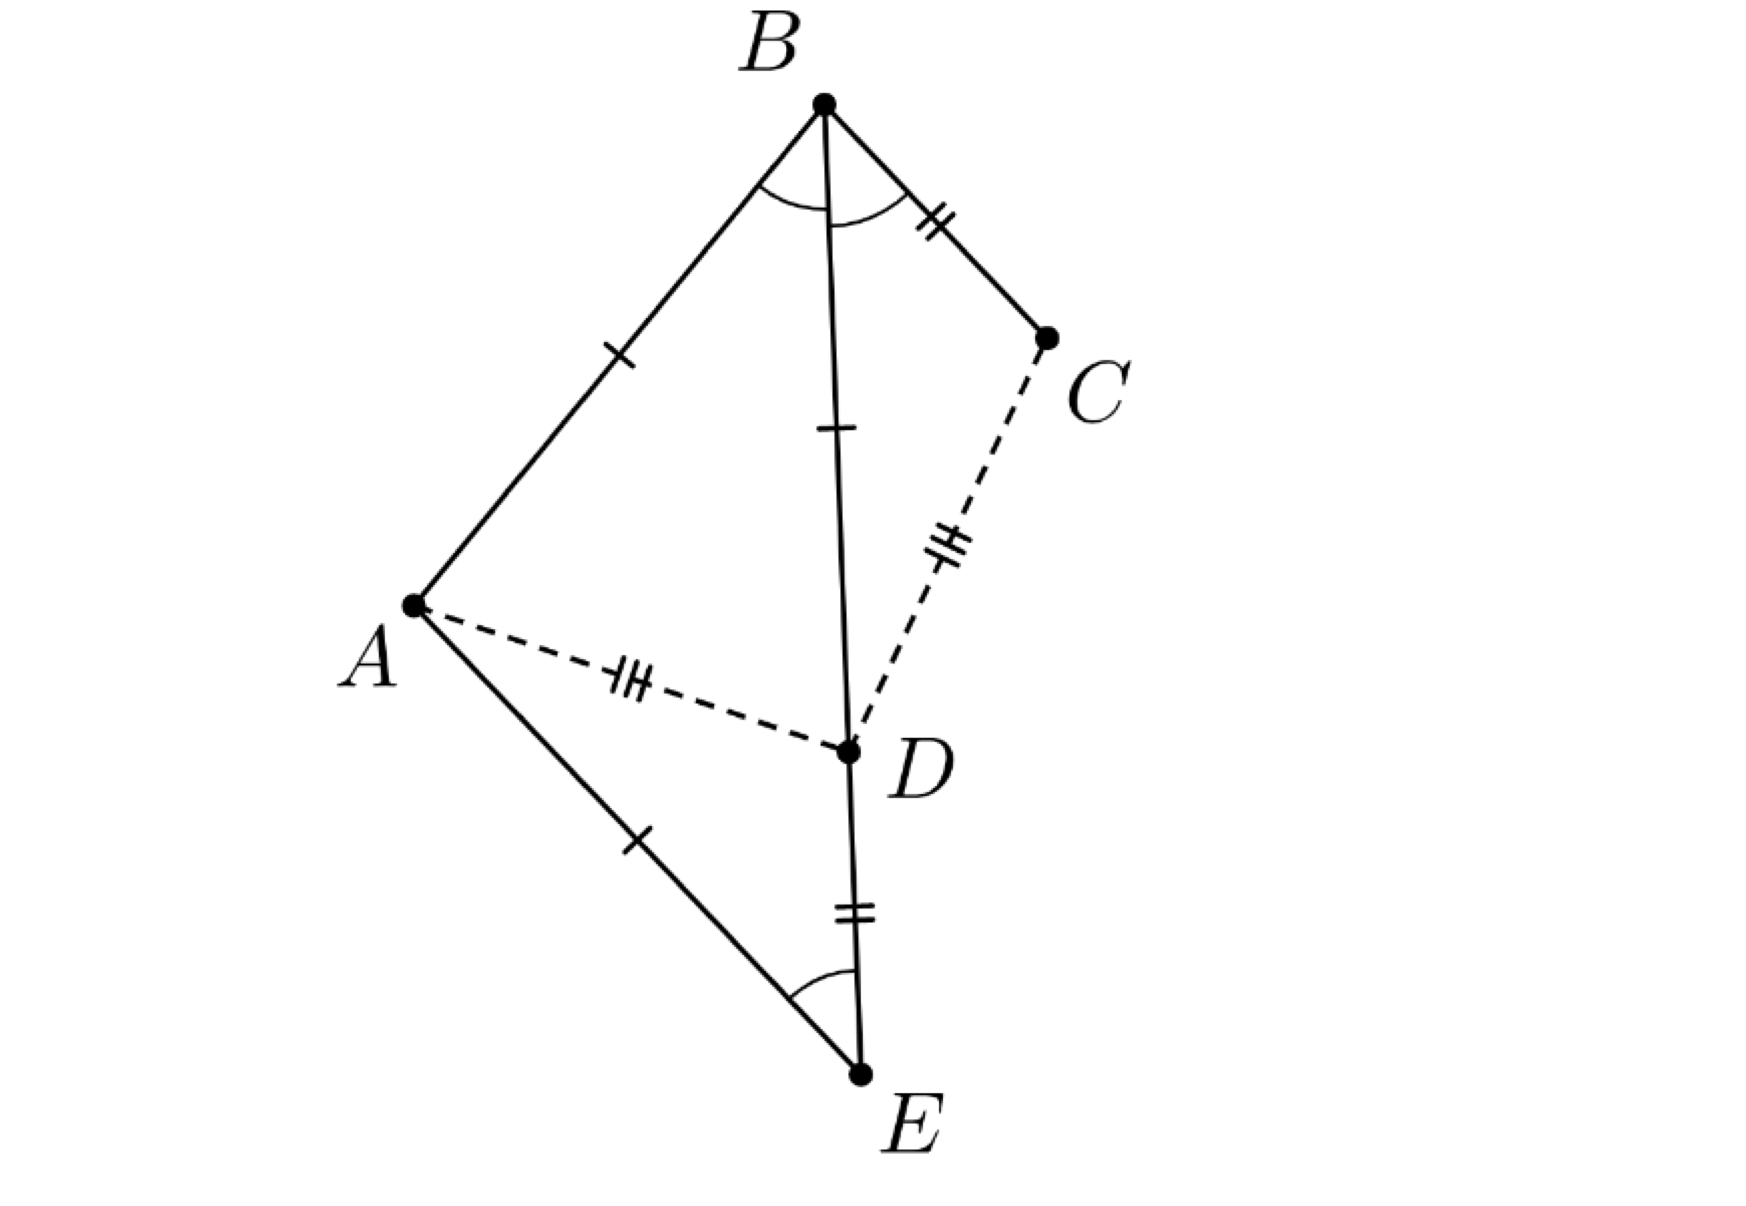
\includegraphics[width=0.5\linewidth]{ЭлМШ 2025-2026//III блок//8//Тренировки//II//Решения/8.2.2.png}
    \caption{}
    \label{fig:placeholder}
\end{figure}

\problem{8.3}
На доске написаны четыре числа: $2,3,4$ и 6 . За один шаг можно выбрать любые три из них, первое умножить на 2 , второе - на 3 , а третье - на 6 (при этом три старых числа стирают, а на их место записывают три новых). Можно ли через несколько шагов получить на доске четыре равных числа?

\textit{Ответ. Нельзя.}

\textit{Решение.}
Произведение изначальных чисел на доске равнялось $2^4 \cdot 3^2$, а после каждой операции оно увеличивается в $2 \cdot 3 \cdot 6=2^2 \cdot 3^2$ раз, поэтому после $n$ таких операций произведение чисел на доске будет равно $2^{4+2 n} \cdot 3^{2+2 n}$. Если после нескольких таких операций получились четыре равных числа, то их произведение имеет вид $2^{4 x} \cdot 3^{4 y}$, для натуральных $x$ и у. Но числа $4+2 n$ и $2+2 n$ не могут одновременно делится на 4, получаем противоречие.

\problem{8.4}
Найдите значение суммы

$$
\begin{gathered}
S=\left(1^2+1 \cdot 2+2^2\right)+\left(2^2+2 \cdot 3+3^2\right)+\left(3^2+3 \cdot 4+4^2\right)+\cdots \\
+\left(98^2+98 \cdot 99+99^2\right)+\left(99^2+99 \cdot 100+100^2\right)
\end{gathered}
$$

\textit{Ответ. $100^3-1^3=999999$.}

\textit{Решение.}
Заметим, что $a^2+a b+b^2=\frac{b^3-a^3}{b-a}$.

Тогда $S=\frac{2^3-1^3}{2-1}+\frac{3^3-2^3}{3-2}+\ldots+\frac{100^3-99^3}{100-99}=100^3-1^3=999999$.

\problem{8.5}
На столе лежат 100 карточек с числами от 1 до 100 . Двое играют в следующую игру. Ходят по очереди. За один ход можно взять со стола любую карточку. Игра заканчивается, когда на столе останется две карточки. Второй выигрывает, если числа на оставшихся карточках отличаются ровно на 10 . Иначе выигрывает первый. Кто выигрывает при правильной игре?

\textit{Ответ. Второй.}

\textit{Решение.}
Опишем стратегию второго игрока. Пусть он разобьет карточки на пары следующим образом: $1-11,2-12,3-13, \ldots, 10-20,21-31,22-32, \ldots, 89-99$, 90-100. Тогда в каждой паре числа отличаются ровно на 10 . Каждым ходом второму игроку следует брать карточку из той пары, из которой только что взял карточку первый игрок. Поэтому после каждого хода второго игрока количество пар будет уменьшаться на одну. В конце игры на столе останется одна пара карточек. Числа в ней отличаются на 10 . Поэтому второй игрок выиграет.